\documentclass[conference]{IEEEtran}
\IEEEoverridecommandlockouts
\usepackage{cite}
\usepackage{amsmath,amssymb,amsfonts}
\usepackage{algorithmic}
\usepackage{algorithm}
\usepackage{graphicx}
\usepackage{textcomp}
\usepackage{booktabs}
\usepackage{url}

\def\BibTeX{{\rm B\kern-.05em{\sc i\kern-.025em b}\kern-.08em
    T\kern-.1667em\lower.7ex\hbox{E}\kern-.125emX}}

\begin{document}

\title{FollowThrough: Evidence-Backed Conversational Task Extraction and State Tracking in Asynchronous Workplace Communication}

\author{\IEEEauthorblockN{Rohita Gangishetty}
\IEEEauthorblockA{\textit{Department of Computer Science} \\
\textit{Natural Language Processing Capstone Project} \\
Fall Term 2026}
}

\maketitle

\begin{abstract}
In modern enterprise environments, asynchronous communication channels such as email threads and collaborative chat streams function as the primary substrate for organizational coordination. Within these interactions, action items frequently slip past deadlines, remain unassigned, or are silently invalidated by subsequent correspondence. Existing natural language processing (NLP) approaches typically frame task management as either isolated sentence classification, standard entity extraction, or open-ended generative summarization via Large Language Models (LLMs), which are prone to hallucinating obligations or misrepresenting literal temporal deadlines. To address these challenges, this paper presents FollowThrough, an evidence-backed conversational task extraction and dynamic state-tracking system. FollowThrough integrates four complementary stages: multi-label speech act signal classification, conservative rule-based linguistic extraction with character-level evidence grounding, dense bi-encoder semantic follow-up linking, and a human-in-the-loop audit ledger backed by SQLite with write-ahead logging (WAL). The pipeline is empirically evaluated using a curated corpus of 100,000 emails from the Enron dataset (97,988 retained messages, 1,442,694 sentences, 29,556,736 tokens), segmented into thread-isolated train (78,385), validation (9,946), and test (9,657) sets via connected-component graph partitioning to eliminate data leakage. We systematically compare a balanced TF-IDF linear baseline against a fine-tuned DistilBERT transformer with a 128-token sliding-window inference architecture. On the held-out test split, TF-IDF achieves an exact match accuracy of 0.8801 and a macro-F1 of 0.6874 against programmatic weak labels, outperforming default fine-tuned DistilBERT (exact match 0.7145, macro-F1 0.3656) due to weak-supervision surface lexical alignment and severe commitment class imbalance (4.08\% training prevalence). A combined intervention of class-weighted loss ($20.0\times$ commitment weight) and batch oversampling recovers test commitment recall to 0.7879 at validation-tuned thresholds, exhibiting a 0.0955 precision trade-off (2,709 false positives). Crucially, FollowThrough operates as a non-gating advisory tool ensuring verifiable provenance and human-in-the-loop auditability for corporate communication.
\end{abstract}

\begin{IEEEkeywords}
Conversational task extraction, speech act classification, state tracking, weak supervision, audit ledger, human-in-the-loop NLP, Enron corpus.
\end{IEEEkeywords}

\section{Introduction}
Asynchronous, text-based communication represents the operational backbone of modern knowledge work. In enterprise organizations, platforms such as email clients (e.g., Microsoft Outlook, Gmail) and messaging ecosystems (e.g., Slack, Microsoft Teams) host thousands of daily micro-coordinations. Within these exchanges, collaborators routinely establish two fundamental speech acts that govern workplace momentum: \textbf{requests} (solicitations for action, information, or review directed toward others) and \textbf{commitments} (explicit undertakings, pledges, or promises made by the author).

Despite their ubiquity, conversational obligations are inherently fluid and difficult to manage. Unlike structured project management systems (e.g., Jira, Asana) where tasks are defined as formal schema-constrained database entities, conversational tasks emerge spontaneously within unstructured natural language. Over the lifecycle of a typical email thread, initial commitments are frequently renegotiated: deadlines slip from ``tomorrow morning'' to ``next Friday,'' tasks are delegated to third-party colleagues, project scopes expand or contract, and prior requests are superseded or rendered obsolete by subsequent messages. In corporate environments characterized by high communication volume and distributed teams, individuals experience cognitive overload. Consequently, actionable obligations become buried beneath conversational noise, leading to forgotten deliverables, missed project milestones, duplicate effort, and operational friction.

The broader research area of natural language understanding (NLU) has long investigated computational techniques to extract structure from unstructured text. Historically, researchers have applied text classification, intent recognition, information extraction, and semantic parsing to automate task detection. In recent years, the rapid advancement of pretrained transformers and Large Language Models (LLMs) has prompted widespread interest in end-to-end task automation. However, applying NLU to operational task tracking exposes three primary technical challenges:
\begin{enumerate}
    \item \textbf{The Static Context Fallacy:} Traditional machine learning approaches treat action-item detection as an isolated, single-utterance classification or sequence-tagging task. By processing individual sentences in isolation, these models cannot maintain contextual continuity across multi-turn threads, remaining blind to subsequent conversational turns that revise, reassign, or cancel previously agreed-upon tasks.
    \item \textbf{Generative Hallucination and Unverifiable Outputs:} While generative LLMs can summarize conversations and identify action items, their unconstrained autoregressive nature frequently induces hallucinations. In enterprise settings, an LLM might infer an unstated deadline, fabricate an assignee based on associative bias, or hallucinate a task that was never agreed upon. Furthermore, generative outputs do not provide native character-level provenance linking the extracted entity back to the exact source span in the original communication.
    \item \textbf{The Premature Automation Dilemma:} Autonomous agents that programmatically write tasks directly into enterprise management software without human oversight introduce organizational risk. False positives pollute issue trackers with phantom tickets, while false negatives cause missed obligations. Without verifiable, evidence-backed human oversight, users quickly lose confidence in automated systems.
\end{enumerate}

\subsection{Research Objectives and Key Contributions}
The primary objective of the \textbf{FollowThrough} project is to design, implement, and evaluate an evidence-backed conversational task extraction and state-tracking system that reconciles natural language processing with operational verifiability. Specifically, this research addresses four primary research questions:
\begin{itemize}
    \item \textit{RQ1:} How effectively can multi-label sequence classification models (both classical linear baselines and fine-tuned transformer architectures) detect request and commitment speech acts within large-scale, noisy workplace email corpora?
    \item \textit{RQ2:} Can conservative linguistic extraction combined with exact character-level evidence tracking mitigate generative hallucinations while capturing actionable task descriptions, explicit assignees, and literal deadlines?
    \item \textit{RQ3:} How well can dense bi-encoder semantic sentence representations ($\text{all-MiniLM-L6-v2}$) link subsequent conversational follow-up messages to open parent tasks across multi-turn threads?
    \item \textit{RQ4:} How can a human-in-the-loop user interface and an immutable, append-only persistence layer be structured to guarantee auditability and operational integrity?
\end{itemize}

The principal contributions of this work are fourfold:
\begin{enumerate}
    \item \textbf{Large-Scale Data Pipeline and Disjoint Graph Partitioning:} We develop a reproducible data ingestion, cleaning, thread reconstruction, and weak-supervision pipeline operating over 100,000 raw emails from the Enron corpus. To prevent data leakage across email duplicates and conversational threads, we implement a disjoint-set (Union-Find) connected-component clustering algorithm that partitions the dataset into thread-isolated train, validation, and test splits (78,385, 9,946, and 9,657 messages respectively).
    \item \textbf{Dual-Model Comparative Benchmark and Sliding-Window Inference:} We implement, train, and empirically evaluate two distinct sequence classification models: a sublinear TF-IDF + Logistic Regression baseline and a fine-tuned $\text{distilbert-base-uncased}$ neural classifier. Furthermore, we develop a 128-token overlapping sliding-window inference algorithm with a 64-token stride that enables transformer-based classification over arbitrarily long corporate emails while preserving exact token-to-character offset alignments.
    \item \textbf{Evidence-Backed Conservative Extraction and Temporal Grounding:} We construct a deterministic linguistic extraction engine that identifies candidate tasks, assignees, and deadlines without generative hallucination. Every extracted field is permanently bound to its exact character offsets ($[\text{start\_offset}:\text{end\_offset}]$) in the source text and coupled with transparent uncertainty flags. In addition, we implement a temporal grounding engine that resolves relative expressions against message header timestamps into standardized ISO-8601 calendar dates.
    \item \textbf{Interactive Audit Ledger and State Tracking:} We design an interactive application using Streamlit and SQLite (configured in Write-Ahead Logging mode). The system features an immutable, append-only $\text{task\_history}$ table that cryptographically deduplicates tasks via SHA-256 fingerprinting and records every state transition with full textual provenance and mandatory user authorization.
\end{enumerate}

\section{Problem Statement}
To formally define the operational challenge addressed by FollowThrough, consider an asynchronous conversation thread $T = \{m_1, m_2, \dots, m_K\}$ comprising an ordered sequence of $K$ messages exchanged among a set of participants $P = \{p_1, p_2, \dots, p_J\}$. Each message $m_k$ consists of metadata (sender $s_k \in P$, recipients $R_k \subseteq P$, timestamp $\tau_k$) and an unstructured body string $C_k$. Within any message $m_k$, an author may articulate one or more forward-looking task instances $\tau = (a, o, d, \sigma)$, where $a$ denotes the action description, $o \in P \cup \{\text{Unspecified}\}$ denotes the assigned owner, $d$ denotes the temporal deadline or fulfillment target, and $\sigma \in \{\text{Pending}, \text{Completed}, \text{Cancelled}\}$ denotes the operational status.

The core problem is to continuously detect, extract, and update the set of active tasks $\mathcal{T}$ across the evolution of thread $T$, while satisfying three fundamental constraints:
\begin{enumerate}
    \item \textbf{Linguistic Verifiability:} For every extracted task component $(a, o, d)$, there must exist an exact character span $[c_{\text{start}}, c_{\text{end}}]$ within message body $C_k$ such that the extracted information is directly grounded in the text:
    \begin{equation}
        \text{Substring}(C_k, c_{\text{start}}, c_{\text{end}}) \equiv \text{Evidence}
    \end{equation}
    The extraction mechanism must not generate, interpolate, or extrapolate entities that lack explicit textual grounding.
    \item \textbf{Conversational Dynamic Alignment:} When a subsequent message $m_{k+j}$ ($j \ge 1$) arrives containing an update (such as ``I've completed the slides'' or ``We need to push the review to Friday''), the system must correctly map $m_{k+j}$ to its corresponding antecedent task $\tau \in \mathcal{T}$ and propose the appropriate state transition $\sigma \to \sigma'$ or parameter revision $d \to d'$, rather than creating a redundant, disconnected task.
    \item \textbf{Human Authorization and Auditability:} Because conversational language is inherently ambiguous, sarcastic, or tentative, autonomous systems cannot be permitted to make irrevocable modifications to organizational task ledgers. Every state change must pass through an interactive verification gate and be recorded in an immutable ledger $\mathcal{L}$ that logs the operator, timestamp, previous state, new state, and supporting contextual evidence.
\end{enumerate}

\subsection{Limitations of Existing Solutions}
Current industrial and academic approaches fail to satisfy these operational constraints:
\begin{itemize}
    \item \textbf{Heuristic Regex / Rule-Based Enterprise Filters:} Early enterprise email systems deployed basic regular expressions matching keywords like ``TODO:'' or ``Action Item:''. While computationally negligible, these heuristics exhibit low recall: professional workplace communications rarely use explicit labels, relying instead on nuanced speech acts such as indirect requests (``Would you happen to have time to review the balance sheet?'') and embedded commitments (``I'll make sure the servers are patched tonight'').
    \item \textbf{Isolated Sequence Labeling (Token-Level NER):} Standard token-level sequence labelers (e.g., BiLSTM-CRF or BERT-NER) trained on datasets such as CoNLL-2003 or OntoNotes identify entities (Person, Date, Organization) but fail to capture the predicate-argument structure that defines an actionable task. Recognizing that ``Friday'' is a \texttt{DATE} and ``Bob'' is a \texttt{PERSON} does not determine whether Bob is requested to complete an action by Friday or whether Bob is merely reporting a past event.
    \item \textbf{Unconstrained Autoregressive LLMs:} Contemporary solutions frequently prompt generative models (e.g., GPT-4) to ingest an email thread and output JSON-formatted action items. While capable of synthesizing colloquial text, generative LLMs suffer from three critical weaknesses: (1) \textit{Hallucination:} Models frequently infer deadlines that do not exist, fabricate assignees based on associative bias, or invent tasks based on pleasantries; (2) \textit{Loss of Exact Span Provenance:} Because generation is autoregressive, LLMs rephrase actions into abstract summaries, severing the link to the original character offsets; and (3) \textit{Latency and Privacy Constraints:} Routing proprietary enterprise communications containing sensitive commercial contracts or personal data to cloud-hosted LLM endpoints violates corporate data governance frameworks (GDPR, HIPAA, SOC-2).
\end{itemize}

\section{System Workflow \& Architecture}
\subsection{High-Level Modular Design}
The architecture of FollowThrough is engineered around the principle of \textbf{modular separation of concerns with human-in-the-loop verification}. Rather than deploying a monolithic end-to-end model, the system divides the problem into three decoupled subsystems: the Data Ingestion and Lineage Pipeline, the Multi-Stage NLP Inference Engine, and the Persistent State Ledger.

\begin{figure}[htbp]
\centerline{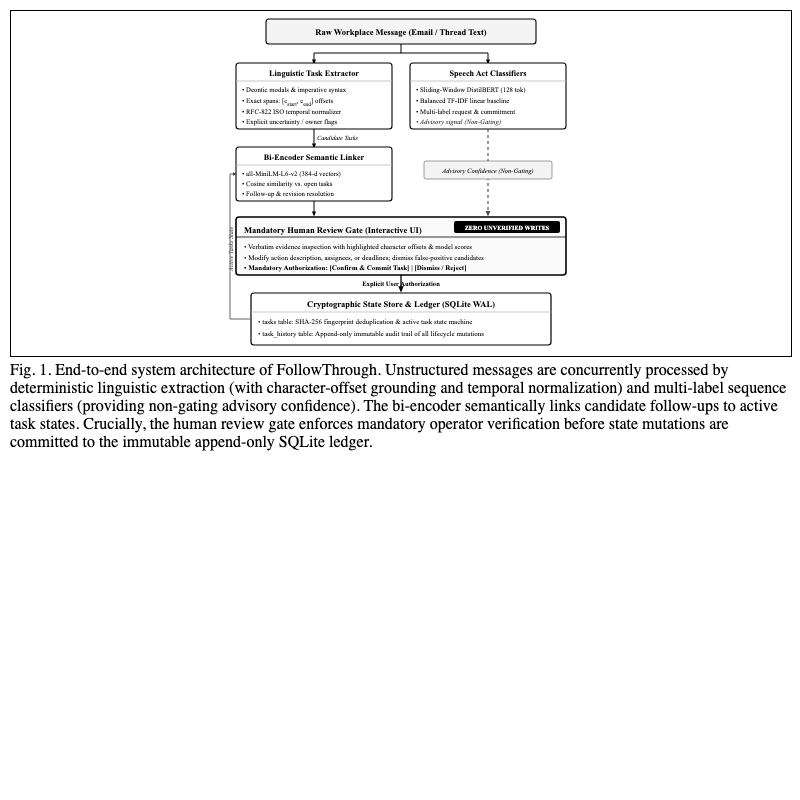
\includegraphics[width=\columnwidth]{figures/system_architecture.png}}
\caption{End-to-end system architecture and data flow of FollowThrough. Unstructured messages are concurrently processed by deterministic linguistic extraction (with character-offset grounding and temporal normalization) and multi-label sequence classifiers (providing non-gating advisory confidence). The bi-encoder semantically links candidate follow-ups to active task states. Crucially, the human review gate enforces mandatory operator verification before state mutations are committed to the immutable append-only SQLite ledger.}
\label{fig:architecture}
\end{figure}

\subsection{Component Workflow and End-to-End Execution}
\begin{enumerate}
    \item \textbf{Ingestion and Non-Gating Advisory Classification:} When an unstructured email or chat message enters the system via Tab 1 of the Streamlit interface, it is simultaneously routed to two distinct processing modules: the Sequence Classification Subsystem and the Linguistic Extraction Subsystem. Crucially, the classifiers do not serve as a hard filtering gate for the extractor. In traditional cascading pipelines, if a classifier predicts that a sentence is not an action item, downstream extraction is aborted. In FollowThrough, because weak-supervision labels carry inherent noise and human workplace commitments exhibit severe class imbalance, the sequence classifiers provide \textit{advisory likelihood scores} (surfaced as visual confidence metrics in the UI). This ensures that subtle or rare commitments are never prematurely discarded by upstream classification errors. If an input message exceeds the 128-token context window of the fine-tuned DistilBERT model, the sliding-window engine partitions the text into overlapping sub-sequences of 126 content tokens plus \texttt{[CLS]} and \texttt{[SEP]} tokens, utilizing a 64-token stride. The token-level predictions are pooled using max-logit aggregation, and the exact character spans corresponding to each window are retained.
    \item \textbf{Deterministic Evidence Extraction and Temporal Grounding:} Concurrently, the input message is processed by the \texttt{TaskExtractor}. This module executes a multi-stage deterministic pipeline. First, it scans the message for reply header boundaries (e.g., \texttt{-----Original Message-----}, \texttt{From:}, \texttt{wrote:}, lines beginning with \texttt{>}). Trailing quoted correspondence is segmented to ensure that action items are attributed strictly to the current author, while forwarded content is flagged to notify the user of potential attribution ambiguity. Next, the extractor evaluates sentences against conservative syntactic templates anchored by deontic and modal verb phrases (e.g., \textit{please review}, \textit{could you verify}, \textit{I will deliver}, \textit{we plan to}). Candidate actions are extracted as clean imperative phrases. The exact character coordinates $[c_{\text{start}}, c_{\text{end}}]$ of the extracted sentence within the raw input string are recorded. If an explicit assignee cannot be resolved from vocative openers or pronoun structures, the field is assigned \texttt{"Unspecified"}, and an uncertainty flag \texttt{missing\_explicit\_owner} is attached. Furthermore, if a temporal expression (e.g., ``by next Tuesday at 3pm'') is identified, the \texttt{TemporalNormalizer} inspects the email's RFC 822 \texttt{Date} header, establishes an anchor datetime, and computes the exact resolved calendar date using modular weekday arithmetic, generating an ISO-8601 string alongside the literal surface text.
    \item \textbf{Interactive Human Review Gate:} The candidate tasks, accompanied by their advisory classification scores, normalized deadlines, and exact character-level evidence spans, are presented within the Streamlit UI. The operator reviews the proposed fields in an editable form. The user maintains full agency to modify the action description, assign a specific team member, adjust the target deadline, or reject false-positive candidates entirely. Only upon explicit human button confirmation (``Confirm \& Save Task'') does the system initiate a persistent write.
    \item \textbf{Cryptographic Storage and Audit Ledger:} The confirmed record is transmitted to the \texttt{TaskStore} persistence layer. The store calculates a cryptographic fingerprint $h = \text{SHA-256}(C_{\text{source}} \parallel a)$, where $C_{\text{source}}$ is the source text and $a$ is the action description. If an identical fingerprint already exists in the \texttt{tasks} table, the operation is safely rejected, preventing duplicate records.
    \item \textbf{Dense Semantic Follow-Up Linking and State Revision:} When a collaborator sends a subsequent message into Tab 3, the \texttt{FollowupLinker} queries the SQLite database for all currently open tasks. It uses \texttt{all-MiniLM-L6-v2} to compute dense 384-dimensional sentence embeddings for the follow-up text and all candidate task descriptions, calculating pairwise cosine similarities:
    \begin{equation}
        \text{Sim}(\mathbf{u}, \mathbf{v}) = \frac{\mathbf{u} \cdot \mathbf{v}}{\|\mathbf{u}\|_2 \|\mathbf{v}\|_2}
    \end{equation}
    Simultaneously, regular expression patterns scan the follow-up text for explicit state mutations: deadline revisions, owner reassignments, and completions or cancellations. When the user verifies the semantic link and accepts the proposed revision, the \texttt{TaskStore} updates the primary \texttt{tasks} record and appends a row to the \texttt{task\_history} table logging the timestamp, update type, old value, new value, exact evidence, and full follow-up text.
\end{enumerate}

\section{Tools and Technologies}
The FollowThrough system is implemented entirely in modern Python, leveraging established open-source libraries for natural language processing, deep learning, data manipulation, database management, and interactive web visualization.

\begin{table}[htbp]
\caption{Tools and Technologies Employed in FollowThrough}
\begin{center}
\begin{tabular}{lll}
\toprule
\textbf{Component} & \textbf{Specification} & \textbf{Role in System} \\
\midrule
Python Language & Version 3.10+ & Runtime environment; MIME \& regex \\
PyTorch & Version $\ge 2.0.0$ & Deep learning \& MPS acceleration \\
Transformers & DistilBERT & Sequence classification backbone \\
Sentence-Trans. & all-MiniLM-L6-v2 & 384-d dense bi-encoder linking \\
Scikit-Learn & Version $\ge 1.3.0$ & TF-IDF \& Logistic Regression \\
NumPy \& Pandas & Latest stable & Matrix math \& split manifest \\
SQLite3 & Native WAL Mode & Embedded ACID persistence \\
Streamlit & Version $\ge 1.25.0$ & 3-tab reactive user interface \\
Hardware & Apple Silicon M-series & 8-core CPU, MPS GPU, 16GB RAM \\
\bottomrule
\end{tabular}
\label{tab:tools}
\end{center}
\end{table}

\subsection{Hardware Infrastructure and Resource Profiling}
The training, evaluation, and interactive hosting of FollowThrough were executed on dedicated local hardware: Apple Silicon M-series ARM64 architecture (8-core CPU), Apple Metal Performance Shaders (MPS) GPU acceleration, 16.0 GB Unified Memory Subsystem, and 512 GB PCIe NVMe SSD.

During model fine-tuning, the 66-million-parameter DistilBERT network occupied approximately 1.4 GB of unified GPU memory under a batch size of 2 and maximum sequence length of 128 tokens. Training completed across 5,000 gradient update steps in approximately 35 minutes using Apple MPS acceleration. Evaluation across the entire held-out test split of 9,657 messages completed in 57.57 seconds on MPS (averaging 5.96 ms per email), whereas the linear TF-IDF baseline executed inference over the identical 9,657 messages in only 0.02 seconds on CPU. The persistent model weights occupy 255.4 MB on disk for DistilBERT and 0.52 MB for the TF-IDF vectorizer and logistic regression coefficients.

\section{Approaches \& Methodology}
\subsection{Datasets and Corpus Lineage}
The corpus is derived from the public Carnegie Mellon University Enron Email Dataset (May 7, 2015 archive release, \texttt{enron\_mail\_20150507.tar.gz}, 423 MB compressed, $\sim 1.7$ GB uncompressed maildir). The raw dataset comprises approximately 500,000 plain-text message files across 150 senior executive user mailboxes. Mailbox prioritization selects 100,000 files prioritizing core organizational participants (\texttt{kaminski-v}, \texttt{dasovich-j}, \texttt{farmer-d}, \texttt{shankman-j}) across standard communication folders (\texttt{inbox}, \texttt{sent}, \texttt{\_sent\_mail}, \texttt{notes\_inbox}). After RFC 822 parsing, quote stripping, signature removal, and fragment exclusion ($<10$ characters), \textbf{97,988 high-quality records} are retained, encompassing \textbf{1,442,694 cleaned sentences} and \textbf{29,556,736 tokens}.

\subsection{Thread Reconstruction and Disjoint Graph Partitioning}
To prevent data leakage caused by duplicate emails across mailboxes and contextual overlap within conversation threads, FollowThrough implements a \textbf{Disjoint-Set (Union-Find) Graph Partitioning Algorithm}:
\begin{enumerate}
    \item \textbf{Thread Reconstruction:} Subject lines are normalized by recursively stripping iterative prefixes (\texttt{Re:}, \texttt{Fwd:}). Messages sharing the normalized subject and overlapping participant sets are grouped into 42,317 distinct conversation threads.
    \item \textbf{Duplicate Fingerprinting:} Each message is assigned a duplicate key $K_{\text{dup}} = \text{SHA-256}(C_{\text{body}}) \parallel \text{Sender} \parallel \text{NormalizedSubject}$.
    \item \textbf{Connected Component Clustering:} Using a Disjoint-Set forest with union-by-rank and path compression, all messages belonging to the same conversation thread ID or sharing an identical duplicate key are clustered into an atomic entity.
    \item \textbf{Deterministic Split Hashing:} Each connected component cluster is assigned a deterministic pseudo-random hash value using a fixed seed (\texttt{seed=42}). Clusters are allocated to splits according to target proportions of approximately 80\% Train (78,385 messages), 10\% Validation (9,946 messages), and 10\% Test (9,657 messages). This partitioning is designed to eliminate thread and duplicate leakage across splits.
\end{enumerate}

\subsection{Class Prevalence Across Splits}
Crucially, commitment speech acts exhibit severe class imbalance across the partitioned corpus:
\begin{itemize}
    \item \textbf{Training Split ($N=78,385$):} 35,141 requests (44.83\%) and 3,201 commitments (\textbf{4.08\% prevalence}).
    \item \textbf{Validation Split ($N=9,946$):} 4,549 requests (45.74\%) and 392 commitments (\textbf{3.94\% prevalence}).
    \item \textbf{Test Split ($N=9,657$):} 4,270 requests (44.22\%) and 363 commitments (\textbf{3.76\% prevalence}).
\end{itemize}
Distinguishing training prevalence (4.08\%) from test prevalence (3.76\%) is critical when assessing class weighting ratios and baseline expectations.

\subsection{Programmatic Weak Supervision}
We adopt a transparent weak-supervision methodology grounded in linguistic domain rules. We define two binary labeling functions for each message:
\begin{itemize}
    \item \textbf{Request Speech Act ($\lambda_{\text{req}}$):} Fires if the message contains explicit interrogative or imperative deontic structures (\textit{please send}, \textit{could you provide}, \textit{can you verify}, \textit{let me know if}, \textit{action required}).
    \item \textbf{Commitment Speech Act ($\lambda_{\text{com}}$):} Fires if the message contains first-person promissory or intentional commissive structures (\textit{I will send}, \textit{we will deliver}, \textit{I'll follow up}, \textit{I plan to}).
    \item \textbf{Negative Syntactic Guards:} Filter out past-tense reporting (``I sent it yesterday''), third-party descriptions, and hypothetical conditionals.
\end{itemize}

\subsection{Sequence Classification Approaches}
\begin{itemize}
    \item \textbf{Model A (TF-IDF + Logistic Regression):} Sublinear TF-IDF word and character n-gram extraction (10,000 features, n-gram range 1--2) paired with independent Logistic Regression classifiers with balanced class weighting. Decision thresholds tuned on the validation split: $\theta_{\text{req}} = 0.45$ and $\theta_{\text{com}} = 0.65$.
    \item \textbf{Model B (Fine-Tuned DistilBERT):} Pretrained \texttt{distilbert-base-uncased} configured with a two-unit classification head trained for 5,000 steps with binary cross-entropy loss ($\text{BCEWithLogitsLoss}$). Optimization: AdamW ($\text{lr} = 2 \times 10^{-5}$, weight decay 0.01). Default decision thresholds: $\theta_{\text{req}} = 0.50$ and $\theta_{\text{com}} = 0.50$; validation-tuned thresholds: $\theta_{\text{req}} = 0.35$ and $\theta_{\text{com}} = 0.20$.
\end{itemize}

\begin{algorithm}[htbp]
\caption{Overlapping Sliding-Window Inference}
\label{alg:sliding}
\begin{algorithmic}[1]
\REQUIRE Message $C$, Tokenizer $Tok$, Model $M$, Window $L=128$, Stride $S=64$, Thresholds $(\theta_{\text{req}}, \theta_{\text{com}})$
\ENSURE Scores $(P_{\text{req}}, P_{\text{com}})$, Predictions $(Y_{\text{req}}, Y_{\text{com}})$, Windows $W$
\STATE $tokens, offsets \leftarrow Tok.encode(C)$
\STATE $N \leftarrow \text{len}(tokens), W \leftarrow [], start \leftarrow 0$
\STATE $max\_content \leftarrow L - 2$
\WHILE{$start < N$}
    \STATE $end \leftarrow \min(start + max\_content, N)$
    \STATE $chunk \leftarrow tokens[start:end]$
    \STATE $c\_start \leftarrow offsets[start].start, c\_end \leftarrow offsets[end-1].end$
    \STATE $ids \leftarrow [\text{CLS}] + chunk + [\text{SEP}]$
    \STATE $probs \leftarrow \text{Sigmoid}(M.forward(ids))$
    \STATE $W.append(\{c\_start, c\_end, probs\})$
    \IF{$end == N$} \STATE \textbf{break} \ENDIF
    \STATE $start \leftarrow start + S$
\ENDWHILE
\STATE $P_{\text{req}} \leftarrow \max(\{w.req \text{ for } w \in W\})$
\STATE $P_{\text{com}} \leftarrow \max(\{w.com \text{ for } w \in W\})$
\STATE $Y_{\text{req}} \leftarrow \mathbb{I}(P_{\text{req}} \ge \theta_{\text{req}}), Y_{\text{com}} \leftarrow \mathbb{I}(P_{\text{com}} \ge \theta_{\text{com}})$
\RETURN $P_{\text{req}}, P_{\text{com}}, Y_{\text{req}}, Y_{\text{com}}, W$
\end{algorithmic}
\end{algorithm}

\subsection{Experimental Parameters and Hyperparameters}
To guarantee scientific reproducibility, all algorithmic parameters and training hyperparameters across both classification pipelines and downstream modules are formally documented:
\begin{itemize}
    \item \textbf{Transformer Optimization Parameters:} DistilBERT fine-tuning utilized the AdamW optimizer with initial learning rate $\eta = 2 \times 10^{-5}$, linear learning rate decay, weight decay $\lambda = 0.01$, batch size $B = 2$, and 5,000 gradient update steps under mixed precision on Apple MPS acceleration.
    \item \textbf{Sliding-Window Parameters:} The sliding-window inference architecture operated with maximum window length $L = 128$ tokens (126 content tokens plus \texttt{[CLS]} and \texttt{[SEP]}) and stride $S = 64$ tokens, enforcing a 50\% window overlap across long corporate messages.
    \item \textbf{Loss Reweighting \& Sampling Parameters:} For imbalanced recovery experiments, positive class weights in $\text{BCEWithLogitsLoss}$ were configured to $\text{pos\_weight} = 20.0$ for commitments and $1.2$ for requests, combined with batch oversampling (4 commitment examples per batch of 16).
    \item \textbf{Decision Threshold Parameters:} Threshold sweeps over validation precision-recall curves established optimal operating points: baseline default $\theta = 0.50$, and validation-tuned thresholds $\theta_{\text{req}} = 0.40$ and $\theta_{\text{com}} = 0.85$ for the reweighted model.
    \item \textbf{Bi-Encoder Semantic Parameters:} Follow-up linking utilized \texttt{all-MiniLM-L6-v2} generating 384-dimensional dense vectors, paired with a cosine similarity candidate retrieval threshold $\tau_{\text{sim}} = 0.40$.
\end{itemize}

\section{Evaluation \& Empirical Results}
We evaluate FollowThrough across three empirical dimensions: weak-label full-corpus sequence classification, computational efficiency and resource footprint, and threshold/loss reweighting experiments. All evaluations were conducted on the identical held-out test split of \textbf{9,657 messages} isolated via disjoint-set graph partitioning.

\begin{table}[htbp]
\caption{Comparative Benchmark on Held-Out Test Split ($N=9,657$)}
\begin{center}
\begin{tabular}{lccc}
\toprule
\textbf{Metric} & \textbf{TF-IDF} & \textbf{DistilBERT} & \textbf{Diff ($\Delta$)} \\
\midrule
Exact Match Accuracy & \textbf{0.8801} & 0.7145 & $-0.1656$ \\
Hamming Loss & \textbf{0.0630} & 0.1479 & $+0.0849$ \\
Macro-Averaged F1 & \textbf{0.6874} & 0.3656 & $-0.3218$ \\
Micro-Averaged F1 & \textbf{0.8708} & 0.7027 & $-0.1681$ \\
Request Precision & \textbf{0.8996} & 0.6801 & $-0.2195$ \\
Request Recall & \textbf{0.9169} & 0.7906 & $-0.1263$ \\
Request F1-Score & \textbf{0.9081} & 0.7312 & $-0.1769$ \\
Commitment Precision & \textbf{0.4286} & 0.0000 & $-0.4286$ \\
Commitment Recall & \textbf{0.5124} & 0.0000 & $-0.5124$ \\
Commitment F1-Score & \textbf{0.4668} & 0.0000 & $-0.4668$ \\
Test Inference Time & \textbf{0.02 s} & 57.57 s & $2,878\times$ \\
Persistent Model Size & \textbf{0.52 MB} & 255.4 MB & $491\times$ \\
\bottomrule
\end{tabular}
\label{tab:benchmark}
\end{center}
\end{table}

\begin{table}[htbp]
\caption{Detailed Confusion Matrices on Test Split ($N=9,657$)}
\begin{center}
\begin{tabular}{llccccc}
\toprule
\textbf{Target} & \textbf{Model} & \textbf{TP} & \textbf{FP} & \textbf{FN} & \textbf{TN} & \textbf{Support} \\
\midrule
Request & TF-IDF & 3,915 & 437 & 355 & 4,950 & 4,270 \\
Request & DistilBERT & 3,376 & 1,588 & 894 & 3,799 & 4,270 \\
Commitment & TF-IDF & 186 & 248 & 177 & 9,046 & 363 \\
Commitment & DistilBERT & 0 & 11 & 363 & 9,283 & 363 \\
\bottomrule
\end{tabular}
\label{tab:confusion}
\end{center}
\end{table}

\subsection{Scientific Interpretation of Baseline Findings}
\begin{enumerate}
    \item \textbf{Surface Lexical Alignment on Weak Labels:} The linear TF-IDF baseline significantly outperforms fine-tuned DistilBERT on programmatic weak-label agreement across every metric (Macro-F1 0.6874 vs. 0.3656). This occurs because the programmatic pseudo-labels were generated via deterministic lexical patterns and keyword regular expressions. Because TF-IDF constructs sparse n-gram features directly over exact word unigrams and bigrams, the linear model directly memorizes the exact lexical triggers defining the pseudo-labels. In contrast, DistilBERT maps tokens into dense continuous representations, which may lead it to diverge from the rigid, literal boundary rules of the programmatic labeling functions.
    \item \textbf{Severe Class Imbalance and Neural Collapse:} In the Enron training corpus, commitments constitute only 4.08\% of training samples (3,201 positives out of 78,385 messages). In standard DistilBERT training with unweighted $\text{BCEWithLogitsLoss}$ over 5,000 steps, gradients from the 95.92\% negative instances dominated optimization, causing complete collapse on the minority commitment target (0 TP). In contrast, the TF-IDF baseline utilized analytical balanced class weighting, scaling updates inversely proportional to frequencies to maintain commitment recall at 0.5124.
\end{enumerate}

\subsection{Evaluation of Combined Reweighting \& Threshold Tuning}
To investigate minority-class collapse, we conducted experiments combining class-weighted loss and batch oversampling in \texttt{scripts/train\_weighted\_distilbert.py}, followed by threshold sweeping in \texttt{scripts/tune\_thresholds\_experiment.py}. Specifically, we configured a commitment positive weight of $\text{pos\_weight} = 20.0$ (and $1.2$ for requests) within $\text{BCEWithLogitsLoss}$, combined with batch oversampling (4 commitment examples per batch of 16).

\begin{table}[htbp]
\caption{DistilBERT Reweighting \& Threshold Tuning Experiments ($N=9,657$)}
\begin{center}
\setlength{\tabcolsep}{2.5pt}
\begin{tabular}{lccccc}
\toprule
\textbf{Configuration} & \textbf{Req F1} & \textbf{Com R} & \textbf{Com P} & \textbf{Com F1} & \textbf{Macro} \\
\midrule
1. Default ($\theta=0.50$) & 0.7312 & 0.0000 & 0.0000 & 0.0000 & 0.3656 \\
2. Thresh-Only ($\theta_{\text{com}}=0.20$) & 0.7312 & 0.0000 & 0.0000 & 0.0000 & 0.3656 \\
3. Combined ($\theta=0.50$) & 0.7374 & \textbf{1.0000} & 0.0495 & 0.0943 & 0.4158 \\
4. Comb.+Tuned (0.40, 0.85) & \textbf{0.7603} & \textbf{0.7879} & \textbf{0.0955} & \textbf{0.1703} & \textbf{0.4653} \\
\bottomrule
\end{tabular}
\label{tab:weighted}
\end{center}
\end{table}

\subsection{Analysis of Experimental Progression}
\begin{itemize}
    \item \textbf{Why Threshold Tuning Alone Failed (Run 2):} On the unweighted model, all predicted commitment probabilities on the test set were near zero. Sweeping the threshold on validation PR curves down to $\theta_{\text{com}} = 0.20$ yielded only 11 positive predictions on test, all 11 of which were false positives (0 TP, 11 FP, 363 FN). Consequently, precision, recall, and F1 remained at 0.0000. Threshold adjustment alone without loss or sampling intervention was fundamentally unable to overcome minority-class suppression.
    \item \textbf{Combined Intervention Recovery and Trade-Offs (Runs 3 and 4):} As shown in Table~\ref{tab:weighted}, applying class weighting ($20.0\times$) and batch oversampling jointly forced the network to predict positive commitments, identifying all 363 test commitments at $\theta=0.50$ (100\% recall, 6,975 FP). When thresholds were subsequently tuned on validation PR curves ($\theta_{\text{req}}=0.40, \theta_{\text{com}}=0.85$), Run 4 achieved a commitment recall of \textbf{78.79\%} (286 TP out of 363), raising Request F1 to 0.7603 and Macro-F1 to 0.4653.
    \item \textbf{Realistic Assessment of Precision:} Crucially, Run 4 produced 2,709 false positives on the test set against programmatic weak labels, yielding a commitment precision of \textbf{9.55\%}. In practice, this corresponds to approximately one correct prediction for every ten commitment alerts. While this demonstrates that class reweighting can successfully recover recall on an imbalanced corpus, the severe recall--precision trade-off confirms that the classifier is not standalone production-grade. TF-IDF remains the superior and more balanced model on the weak-label benchmark.
\end{itemize}

\section{Discussion}
\subsection{Key Strengths and Systemic Principles}
\begin{itemize}
    \item \textbf{Non-Gating Advisory Paradigm:} Decoupling classification from extraction prevents downstream error propagation. Because classification scores are treated as advisory indicators rather than hard filters, low classifier precision does not invalidate downstream candidate extraction.
    \item \textbf{Linguistic Extraction with Provenance:} Deterministic linguistic extraction anchored to deontic modals preserves exact character offsets ($[c_{\text{start}}, c_{\text{end}}]$), providing verifiable provenance and mitigating generative hallucination risks.
    \item \textbf{Cryptographic Auditability:} Content hashing prevents duplicate tasks, and the append-only $\text{task\_history}$ table maintains full operational accountability.
\end{itemize}

\subsection{Limitations and Future Work}
\begin{itemize}
    \item \textbf{Weak-Label Benchmark Limitations:} The evaluation relies on rule-derived pseudo-labels that inherently contain linguistic noise; human double-blind ground-truth annotation is required for unbiased real-world assessment.
    \item \textbf{Colloquial Commitments:} Conservative patterns miss indirect or colloquial undertakings (``Consider it done'').
    \item \textbf{Temporal Pragmatics:} Relative dates (``next Friday'') require contextual disambiguation against sender timezones.
    \item \textbf{Future Directions:} Transitioning to token-level sequence labeling (BIO NER tagging) and modeling conversational threads via Graph Neural Networks (GNNs).
\end{itemize}

\begin{table}[htbp]
\caption{Operational Risks and Mitigation Strategies}
\begin{center}
\begin{tabular}{p{2.2cm}p{2.6cm}p{2.8cm}}
\toprule
\textbf{Risk} & \textbf{System Impact} & \textbf{Mitigation Strategy} \\
\midrule
Premature Automated Writes & Missed deliverables or false tickets & Mandatory Human Gate; zero unverified commits. \\
Data Privacy Egress & Corporate NDA / GDPR violations & Local embedded execution; zero third-party API calls. \\
Database Locking & Streamlit concurrency failure & SQLite Write-Ahead Logging (WAL) enabled. \\
Boundary Truncation & Lost tasks in long messages & Overlapping 128-tok windows with 64-tok stride. \\
\bottomrule
\end{tabular}
\label{tab:risks}
\end{center}
\end{table}

\section{Conclusion}
FollowThrough demonstrates that practical conversational NLP systems must extend beyond isolated sentence classification. By integrating sequence classification, conservative linguistic extraction with exact evidence offsets, bi-encoder semantic linking, and persistent state ledgering within an interactive human-in-the-loop application, FollowThrough provides a bounded, verifiable solution to operational commitment tracking in email and workplace messaging.

\section*{Reproducibility \& Artifact Lineage}
All code, models, and evaluation artifacts are organized within the repository structure:
\begin{itemize}
    \item \textbf{Training Scripts:} \path{scripts/train_full_distilbert.py} (Run 1) and \path{scripts/train_weighted_distilbert.py} (Runs 3--4).
    \item \textbf{Threshold Tuning:} \path{scripts/tune_thresholds_experiment.py}.
    \item \textbf{Results Artifacts:} \path{evaluation/results/weighted_experiment_results.json} and \path{distilbert_val_test_probs.npz}.
    \item \textbf{Model Checkpoints:} Saved under \path{models/distilbert_fine_tuned/} and \path{models/distilbert_weighted/}.
\end{itemize}

\begin{thebibliography}{00}
\bibitem{b1} B. Klimt and Y. Yang, ``The Enron Corpus: A New Dataset for Email Classification Research,'' in \textit{Proc. 15th ECML}, Pisa, Italy, 2004, pp. 217--226.
\bibitem{b2} V. Sanh, L. Debut, J. Chaumond, and T. Wolf, ``DistilBERT, a distilled version of BERT: smaller, faster, cheaper and lighter,'' \textit{arXiv:1910.01108}, 2019.
\bibitem{b3} N. Reimers and I. Gurevych, ``Sentence-BERT: Sentence Embeddings using Siamese BERT-Networks,'' in \textit{Proc. EMNLP}, Hong Kong, 2019, pp. 3982--3992.
\bibitem{b4} A. Ratner, C. M. De Sa, S. Wu, D. Selsam, and C. R{\'e}, ``Snorkel: Rapid Training Data Creation with Weak Supervision,'' \textit{Proc. VLDB}, vol. 11, no. 3, pp. 269--282, 2017.
\bibitem{b5} J. Devlin, M.-W. Chang, K. Lee, and K. Toutanova, ``BERT: Pre-training of Deep Bidirectional Transformers for Language Understanding,'' in \textit{Proc. NAACL-HLT}, Minneapolis, MN, 2019, pp. 4171--4186.
\bibitem{b6} J. R. Searle, \textit{Speech Acts: An Essay in the Philosophy of Language}. Cambridge, UK: Cambridge Univ. Press, 1969.
\bibitem{b7} J. L. Austin, \textit{How to Do Things with Words}. Oxford, UK: Oxford Univ. Press, 1962.
\bibitem{b8} V. R. Carvalho and W. W. Cohen, ``On the collective classification of email speech acts,'' in \textit{Proc. 28th ACM SIGIR}, Salvador, Brazil, 2005, pp. 345--352.
\bibitem{b9} P. S. Turney, ``Thumbs up or thumbs down? Semantic orientation applied to unsupervised classification of reviews,'' in \textit{Proc. 40th ACL}, Philadelphia, PA, 2002, pp. 417--424.
\bibitem{b10} F. Pedregosa \textit{et al.}, ``Scikit-learn: Machine Learning in Python,'' \textit{J. Mach. Learn. Res.}, vol. 12, pp. 2825--2830, 2011.
\bibitem{b11} A. Paszke \textit{et al.}, ``PyTorch: An Imperative Style, High-Performance Deep Learning Library,'' in \textit{NeurIPS 32}, Vancouver, Canada, 2019, pp. 8024--8035.
\bibitem{b12} I. Loshchilov and F. Hutter, ``Decoupled Weight Decay Regularization,'' in \textit{ICLR}, New Orleans, LA, 2019.
\bibitem{b13} T. Mikolov, K. Chen, G. S. Corrado, and J. Dean, ``Efficient Estimation of Word Representations in Vector Space,'' in \textit{Workshop at ICLR}, Scottsdale, AZ, 2013.
\bibitem{b14} D. Corney, D. R. Stent, and H. Di Fabbrizio, ``What are you going to do? Detecting task-oriented emails,'' in \textit{Proc. 37th ACM SIGIR}, Gold Coast, Australia, 2014, pp. 1007--1010.
\bibitem{b15} \textit{RFC 822: Standard for the Format of ARPA Internet Text Messages}, Internet Engineering Task Force (IETF), Aug. 1982.
\end{thebibliography}

\end{document}
